%%%%%%%%%%%%%%%%%%%%%%%%%%%%%%%%%%%%%%%%%
% Beamer Presentation
% LaTeX Template
% Version 2.0 (March 8, 2022)
%
% This template originates from:
% https://www.LaTeXTemplates.com
%
% Author:
% Vel (vel@latextemplates.com)
%
% License:
% CC BY-NC-SA 4.0 (https://creativecommons.org/licenses/by-nc-sa/4.0/)
%
%%%%%%%%%%%%%%%%%%%%%%%%%%%%%%%%%%%%%%%%%

%----------------------------------------------------------------------------------------
%	PACKAGES AND OTHER DOCUMENT CONFIGURATIONS
%----------------------------------------------------------------------------------------

\documentclass[
	11pt, % Set the default font size, options include: 8pt, 9pt, 10pt, 11pt, 12pt, 14pt, 17pt, 20pt
	%t, % Uncomment to vertically align all slide content to the top of the slide, rather than the default centered
	%aspectratio=169, % Uncomment to set the aspect ratio to a 16:9 ratio which matches the aspect ratio of 1080p and 4K screens and projectors
]{beamer}

\graphicspath{{Images/}{./}} % Specifies where to look for included images (trailing slash required)

\usepackage{booktabs} % Allows the use of \toprule, \midrule and \bottomrule for better rules in tables

%----------------------------------------------------------------------------------------
%	SELECT LAYOUT THEME
%----------------------------------------------------------------------------------------

% Beamer comes with a number of default layout themes which change the colors and layouts of slides. Below is a list of all themes available, uncomment each in turn to see what they look like.

%\usetheme{default}
%\usetheme{AnnArbor}
%\usetheme{Antibes}
%\usetheme{Bergen}
%\usetheme{Berkeley}
%\usetheme{Berlin}
%\usetheme{Boadilla}
%\usetheme{CambridgeUS}
%\usetheme{Copenhagen}
%\usetheme{Darmstadt}
%\usetheme{Dresden}
%\usetheme{Frankfurt}
%\usetheme{Goettingen}
%\usetheme{Hannover}
%\usetheme{Ilmenau}
%\usetheme{JuanLesPins}
%\usetheme{Luebeck}
\usetheme{Madrid}
%\usetheme{Malmoe}
%\usetheme{Marburg}
%\usetheme{Montpellier}
%\usetheme{PaloAlto}
%\usetheme{Pittsburgh}
%\usetheme{Rochester}
%\usetheme{Singapore}
%\usetheme{Szeged}
%\usetheme{Warsaw}

%----------------------------------------------------------------------------------------
%	SELECT COLOR THEME
%----------------------------------------------------------------------------------------

% Beamer comes with a number of color themes that can be applied to any layout theme to change its colors. Uncomment each of these in turn to see how they change the colors of your selected layout theme.

%\usecolortheme{albatross}
%\usecolortheme{beaver}
%\usecolortheme{beetle}
%\usecolortheme{crane}
%\usecolortheme{dolphin}
%\usecolortheme{dove}
%\usecolortheme{fly}
%\usecolortheme{lily}
%\usecolortheme{monarca}
%\usecolortheme{seagull}
%\usecolortheme{seahorse}
%\usecolortheme{spruce}
%\usecolortheme{whale}
%\usecolortheme{wolverine}

%----------------------------------------------------------------------------------------
%	SELECT FONT THEME & FONTS
%----------------------------------------------------------------------------------------

% Beamer comes with several font themes to easily change the fonts used in various parts of the presentation. Review the comments beside each one to decide if you would like to use it. Note that additional options can be specified for several of these font themes, consult the beamer documentation for more information.

\usefonttheme{default} % Typeset using the default sans serif font
%\usefonttheme{serif} % Typeset using the default serif font (make sure a sans font isn't being set as the default font if you use this option!)
%\usefonttheme{structurebold} % Typeset important structure text (titles, headlines, footlines, sidebar, etc) in bold
%\usefonttheme{structureitalicserif} % Typeset important structure text (titles, headlines, footlines, sidebar, etc) in italic serif
%\usefonttheme{structuresmallcapsserif} % Typeset important structure text (titles, headlines, footlines, sidebar, etc) in small caps serif

%------------------------------------------------

%\usepackage{mathptmx} % Use the Times font for serif text
\usepackage{palatino} % Use the Palatino font for serif text

%\usepackage{helvet} % Use the Helvetica font for sans serif text
\usepackage[default]{opensans} % Use the Open Sans font for sans serif text
%\usepackage[default]{FiraSans} % Use the Fira Sans font for sans serif text
%\usepackage[default]{lato} % Use the Lato font for sans serif text

%----------------------------------------------------------------------------------------
%	SELECT INNER THEME
%----------------------------------------------------------------------------------------

% Inner themes change the styling of internal slide elements, for example: bullet points, blocks, bibliography entries, title pages, theorems, etc. Uncomment each theme in turn to see what changes it makes to your presentation.

%\useinnertheme{default}
\useinnertheme{circles}
%\useinnertheme{rectangles}
%\useinnertheme{rounded}
%\useinnertheme{inmargin}

%----------------------------------------------------------------------------------------
%	SELECT OUTER THEME
%----------------------------------------------------------------------------------------

% Outer themes change the overall layout of slides, such as: header and footer lines, sidebars and slide titles. Uncomment each theme in turn to see what changes it makes to your presentation.

%\useoutertheme{default}
%\useoutertheme{infolines}
%\useoutertheme{miniframes}
%\useoutertheme{smoothbars}
%\useoutertheme{sidebar}
%\useoutertheme{split}
%\useoutertheme{shadow}
%\useoutertheme{tree}
%\useoutertheme{smoothtree}

%\setbeamertemplate{footline} % Uncomment this line to remove the footer line in all slides
%\setbeamertemplate{footline}[page number] % Uncomment this line to replace the footer line in all slides with a simple slide count

%\setbeamertemplate{navigation symbols}{} % Uncomment this line to remove the navigation symbols from the bottom of all slides

%----------------------------------------------------------------------------------------
%	PRESENTATION INFORMATION
%----------------------------------------------------------------------------------------

\title[Computer \& Programming, MATLAB]{ENGR1510J Recitation Class} % The short title in the optional parameter appears at the bottom of every slide, the full title in the main parameter is only on the title page

\subtitle{Week 4} % Presentation subtitle, remove this command if a subtitle isn't required

\author[Su Qijian]{Su Qijian} % Presenter name(s), the optional parameter can contain a shortened version to appear on the bottom of every slide, while the main parameter will appear on the title slide

\institute[UM-SJTU JI]{UM-SJTU Joint Institute} % Your institution, the optional parameter can be used for the institution shorthand and will appear on the bottom of every slide after author names, while the required parameter is used on the title slide and can include your email address or additional information on separate lines

\date[\today]{Communication, Computer \& Programming, MATLAB scripting \\ \vspace{1cm} \today} % Presentation date or conference/meeting name, the optional parameter can contain a shortened version to appear on the bottom of every slide, while the required parameter value is output to the title slide

%----------------------------------------------------------------------------------------

\begin{document}

%----------------------------------------------------------------------------------------
%	TITLE SLIDE
%----------------------------------------------------------------------------------------

\begin{frame}
	\titlepage % Output the title slide, automatically created using the text entered in the PRESENTATION INFORMATION block above
\end{frame}

%----------------------------------------------------------------------------------------
%	TABLE OF CONTENTS SLIDE
%----------------------------------------------------------------------------------------

% The table of contents outputs the sections and subsections that appear in your presentation, specified with the standard \section and \subsection commands. You may either display all sections and subsections on one slide with \tableofcontents, or display each section at a time on subsequent slides with \tableofcontents[pausesections]. The latter is useful if you want to step through each section and mention what you will discuss.

\begin{frame}
	\frametitle{Presentation Overview} % Slide title, remove this command for no title
	
	\tableofcontents % Output the table of contents (all sections on one slide)
	%\tableofcontents[pausesections] % Output the table of contents (break sections up across separate slides)
\end{frame}

%----------------------------------------------------------------------------------------
%	PRESENTATION BODY SLIDES
%----------------------------------------------------------------------------------------

\section{Communication} % Sections are added in order to organize your presentation into discrete blocks, all sections and subsections are automatically output to the table of contents as an overview of the talk but NOT output in the presentation as separate slides

%------------------------------------------------

\subsection{Reminders}

\begin{frame}
	\frametitle{Reminders}
 
	\begin{itemize}
    \item RC will be held only on \textbf{Thursday} from \textbf{20:30 to 22:00}.
    \item Recording will be provided.
    \item RC will only review playbooks and solve the worksheet, \textbf{no new content} will be introduced.
    \item We will focus on \textbf{hard questions} from the playbook to optimize RC time. Ensure you are \textbf{familiar with all playbook answers} for exam preparation.
    \item RC will only give ideas on how to solve the worksheet (e.g., pseudo-code), but \textbf{NO direct answers} will be provided in the RC.
    \item A makeup RC for \textbf{Week 2} will be provided \textbf{tomorrow from 20:30 to 22:00}. The makeup RC will be \textbf{online}, and a recording will also be provided in case it conflicts with your schedule.
\end{itemize}

\end{frame}

%------------------------------------------------


\begin{frame}
	\frametitle{Recording}
 
	\begin{itemize}
    \item Recording for RC-1: \href{https://sjtu.feishu.cn/minutes/obcn81s8v371bg9k42p1228p?from_source=finish_recording}{[Link]}.
\end{itemize}

\end{frame}

%------------------------------------------------


\subsection{Communication}

\begin{frame}
	\frametitle{Canvas}
 
	\begin{itemize}
    \item The official resource platform.
    \item Everything related to assignment notifications, timeline announcements, 
    \item Documents, quizzes, and surveys will be posted on \textbf{Canvas}.
    \item Set up your Canvas notifications and settings properly.
    \item Check course files.
    \item You just need to submit your regular homework and projects through \textbf{Gitea}, no need to submit them on Canvas unless it tells you to do so.
\end{itemize}

\end{frame}
%------------------------------------------------


\begin{frame}
	\frametitle{Mattermost}
 
	\begin{itemize}
    \item The official instant message platform.
    \item For general discussions and short questions.
    \item Channels each have their own purpose and offer guidance in their description headers.
    \item Asking questions in the \textbf{Course Question} channel and the individual channel is more advised.
    \item No screenshots if they are not necessary.
    \item Do not post your code in any public channel; provide a link to your code instead.
\end{itemize}

\end{frame}


%-----------------------------------------------
\begin{frame}
	\frametitle{Wechat}
 
	\begin{itemize}
    \item Not official communication tools used in \textbf{ENGR1510J}.
    \item Direct requests on \textbf{WeChat} will be ignored.
    \item Please contact us using tools other than \textbf{WeChat}.
\end{itemize}

\end{frame}

%------------------------------------------------


\begin{frame}
	\frametitle{Email}
 
	\begin{itemize}
    \item Used in the case of a serious project/homework-related concern or personal issue that needs to be discussed privately.
    \item Use brackets \textbf{[ENGR151]} and then include your full name in the subject line of the email.
\end{itemize}

\end{frame}


%------------------------------------------------


\begin{frame}
	\frametitle{Gitea}
 
	\begin{itemize}
    \item Your homework and projects should be uploaded to your \textbf{Gitea repository}.
    \item Set up your \textbf{Gitea account} as well as your \textbf{SSH key}.
\end{itemize}

\end{frame}

%------------------------------------------------

\subsection{Git Usage}

\begin{frame}
	\frametitle{Git Workflow}
	
	\begin{figure}
		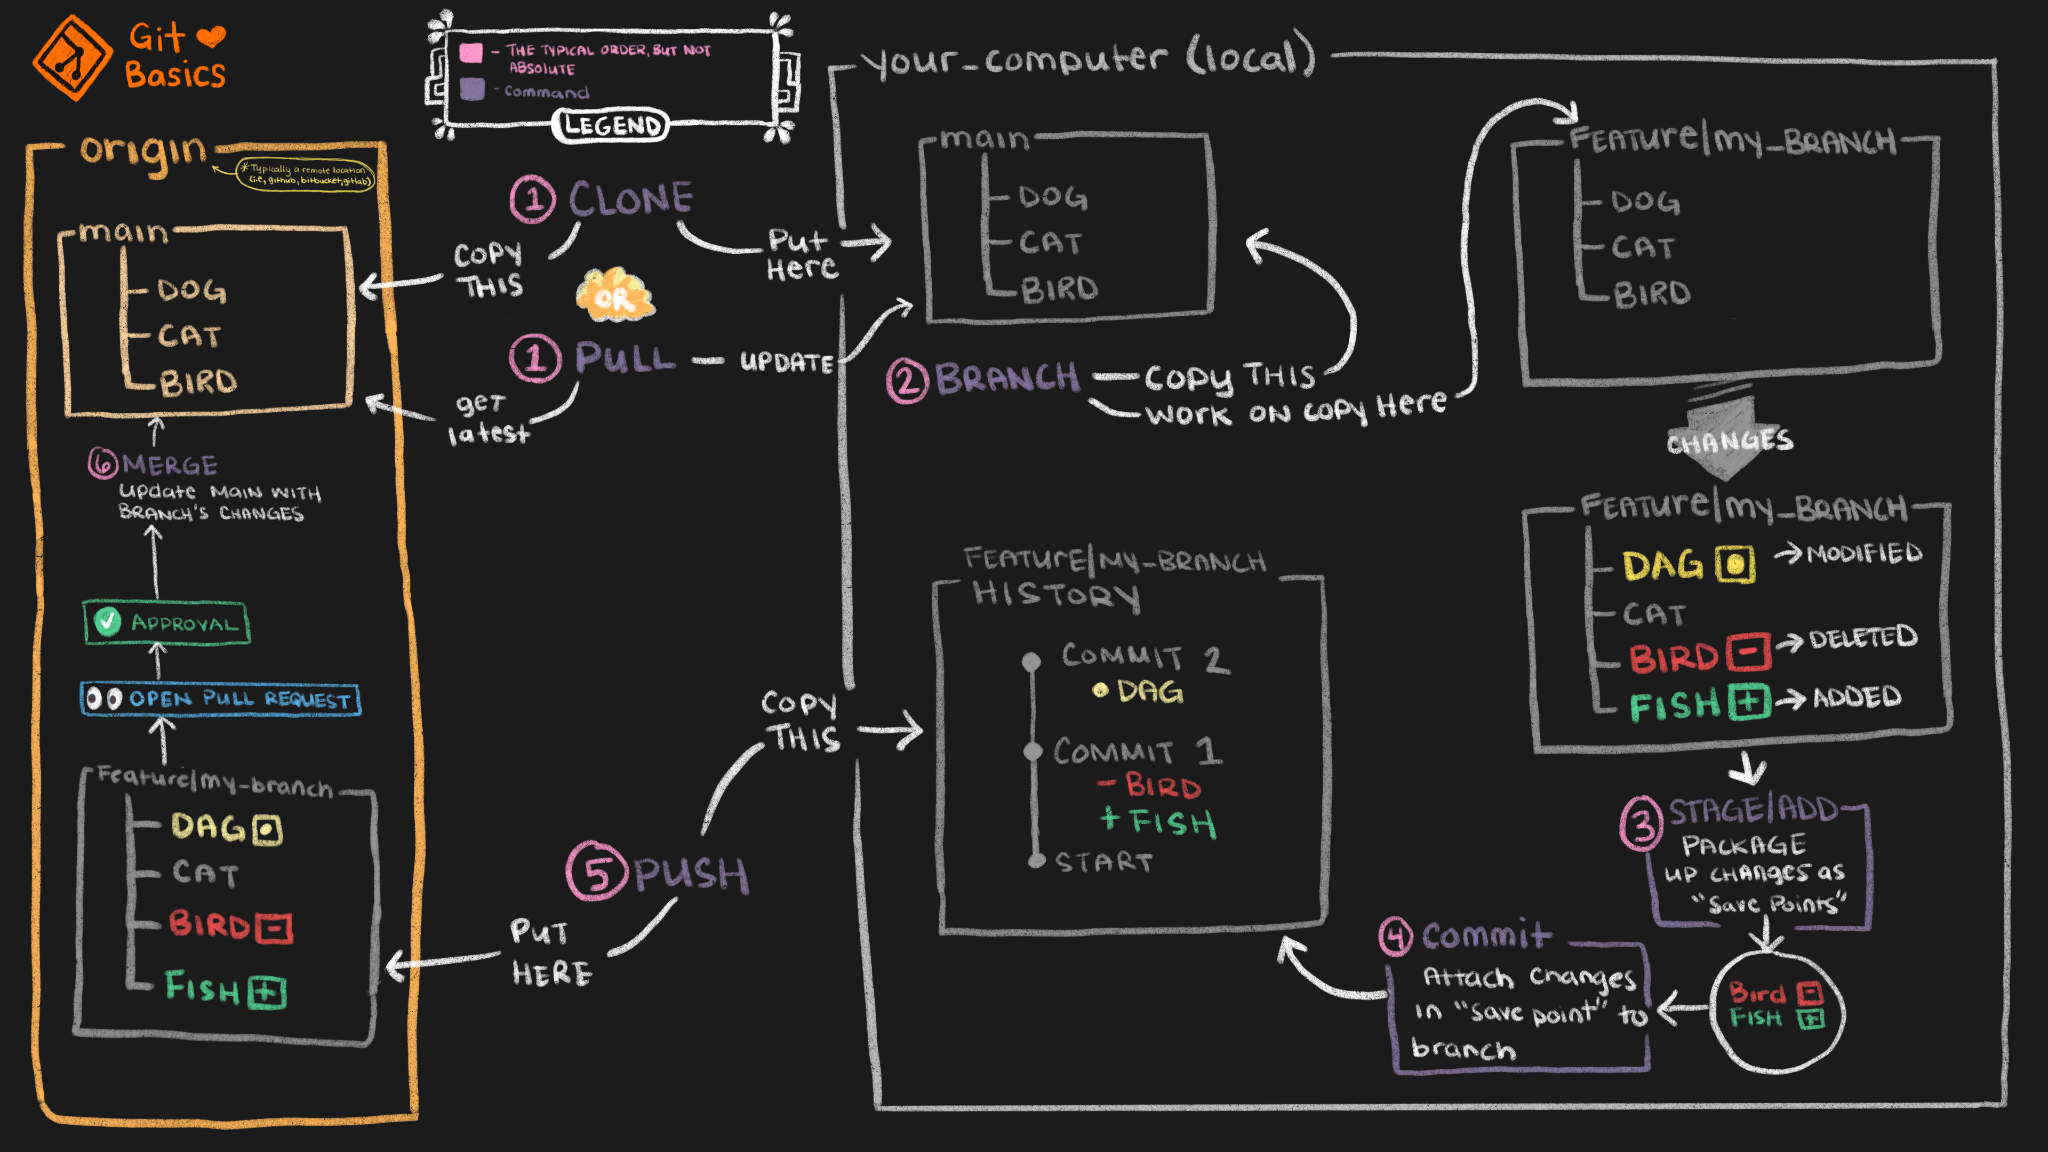
\includegraphics[width=0.8\linewidth]{git_workflow.png}
		\caption{Git Workflow.\footnote{Source: https://www.getdbt.com/analytics-engineering/transformation/git-workflow}}
	\end{figure}
\end{frame}

%------------------------------------------------
\begin{frame}
	\frametitle{Commits}
 
	\begin{itemize}
    \item Commits should be used for saving meaningful changes in the project.
    \item Avoid force commits or using \texttt{git push --force}, as this can overwrite work done by others. A deduction will be applied if you force push without an appropriate reason.
    \item Follow the provided file structure format in the submission.
    \item \textbf{DO NOT directly modify files on Gitea}.
\end{itemize}

\end{frame}
%------------------------------------------------


\begin{frame}
	\frametitle{Issues}
 
	\begin{itemize}
    \item Open an issue in \textbf{Gitea} if you encounter any code-related problems.
    \item Remember to tick the checkbox in issues once you finish the task of each milestone (e.g. your project).
    \item Close the issue once you finish the task or the issue is resolved.
\end{itemize}

\end{frame}
%------------------------------------------------



\begin{frame}
	\frametitle{Pull Requests}
 
	\begin{itemize}
    \item Follow the instructions stated in the course support wiki.
    \item Remember to review and comment on the pull requests and your teammates' code.
    \item Please do not contain any Chinese characters in both your commits and pull request comments.
    \item Approve pull requests as soon as possible if everything is ready (review, comments, debugging). Emergency situations often arise, especially near deadlines!
\end{itemize}

\end{frame}
%------------------------------------------------



\begin{frame}
	\frametitle{Releases}
 
	\begin{itemize}
    \item Remember to create a release for each submission or else a heavy deduction will be applied.
    \item Use the correct release tag for each release.
    \item Please remember to release from the \textbf{master branch}.
\end{itemize}

\end{frame}

%------------------------------------------------

\section{Playbook Review}

\begin{frame}
	\frametitle{Playbook Review}

	\textbf{Disclaimer:} The answers provided here are not guaranteed to be correct. Please use them as a reference only and verify with reliable sources.


\end{frame}

%------------------------------------------------

\subsection{c1}

\begin{frame}
	\frametitle{Review: c1}

	\textbf{Q1: What is Linux?}

	\begin{itemize}
	    \item Linux is an open-source, Unix-like operating system kernel that forms the core of many operating systems.
	\end{itemize}

	\vspace{0.5cm}
	
	\textbf{Q2: Why is Linux important when studying CSE (Computer Science, Computer Engineering, and Software Engineering)?}

	\begin{itemize}
	    \item Linux is widely used in industry, especially in server environments and development.
	    \item Many programming tools, such as compilers, debuggers, and version control systems, are built around or perform better in Linux.
	\end{itemize}

\end{frame}

%------------------------------------------------

\begin{frame}
	\frametitle{Review: c1}

	\textbf{Q3: Can a device do both input and output?}

	\begin{itemize}
	    \item Yes, such as touchscreen or network cards.
	\end{itemize}

	\vspace{0.5cm}

	\textbf{Q4: What are the CPU and the RAM?}

	\begin{itemize}
	    \item \textbf{CPU (Central Processing Unit):}
	    \begin{itemize}
	        \item It performs calculations and executes instructions to run programs.
	        \item It consists of two main components: the arithmetic logic unit (ALU), which performs mathematical operations, and the control unit, which directs operations within the computer.
	    \end{itemize}
	    
	    \item \textbf{RAM (Random Access Memory):}
	    \begin{itemize}
	        \item RAM is a type of computer memory that stores data and machine code currently being used.
	        \item It is volatile, meaning that it only retains information while the computer is powered on.
	    \end{itemize}
	\end{itemize}

\end{frame}

%------------------------------------------------


\begin{frame}
	\frametitle{Review: c1}

	\textbf{Q5: What is the usage of a programming language?}

	\begin{itemize}
	    \item A programming language is a formal language used to write instructions for a computer to execute.
	\end{itemize}

	\vspace{0.5cm}

	\textbf{Q6: Why do we need to be very specific when writing an algorithm?}

	\begin{itemize}
	    \item Being specific ensures that the algorithm covers all possible cases and handles edge conditions effectively.
	    \item Clear, specific instructions help other developers understand and maintain the code.
	\end{itemize}

\end{frame}

%------------------------------------------------


\begin{frame}
	\frametitle{Review: c1}

    \label{slide:q7}

\textbf{Q7: What is the difference between interpreted and compiled languages?}
	\begin{itemize}
	    \item \textbf{Interpreted Languages:}
	    \begin{itemize}
	        \item Code is executed line by line by an interpreter at runtime.
	        \item No need for a separate compilation step.
	        \item Slower execution due to real-time interpretation.
	    \end{itemize}
	    
	    \item \textbf{Compiled Languages:}
	    \begin{itemize}
	        \item Code is converted into machine code by a compiler before execution.
	        \item Faster execution because the code is precompiled into a binary format.
	        \item Requires a separate compilation step before running the program.
	    \end{itemize}
	\end{itemize}


\end{frame}

%------------------------------------------------


\begin{frame}
	\frametitle{Review: c1}

	\textbf{Q8: What are "high-level" and "low-level" programming languages?}

	\begin{itemize}
	    \item \textbf{High-Level Languages:}
	    \begin{itemize}
	        \item Closer to human languages, abstracting away most of the hardware details.
	        \item Easier to read, write, and maintain.
	    \end{itemize}
	    
	    \item \textbf{Low-Level Languages:}
	    \begin{itemize}
	        \item Closer to machine code, providing little to no abstraction from the hardware.
	        \item More efficient in terms of execution but harder to understand and write.
	    \end{itemize}
	\end{itemize}

\end{frame}

%------------------------------------------------

\begin{frame}
	\frametitle{Review: c1}

\textbf{Q9: What is MATLAB good at?}

	\begin{itemize}
	    \item MATLAB is highly efficient for numerical computations, data analysis, and algorithm development, making it ideal for engineering, scientific, and mathematical applications.
	\end{itemize}

	\vspace{0.5cm}

	\textbf{Q10: Why should the input and output always be clearly defined?}

	\begin{itemize}
	    \item It avoids ambiguity, making it easier to verify correctness and troubleshoot errors.
	    \item Clear definitions improve communication and collaboration between developers, helping ensure that the program meets user requirements.
	    \item It also helps in maintaining code and facilitating future updates or modifications.
	\end{itemize}
	

\end{frame}

%------------------------------------------------



\begin{frame}
	\frametitle{Review: c1}

	\textbf{Q11: What is the difference between a mathematical and a physical solution?}

	\begin{itemize}
	    \item \textbf{Mathematical Solution:}
	    \begin{itemize}
	        \item A solution derived purely from mathematical models and equations. 
            \item It may involve idealized assumptions that simplify the problem for analysis.
	    \end{itemize}
	    
	    \item \textbf{Physical Solution:}
	    \begin{itemize}
	        \item A solution that is physically realizable and accounts for real-world constraints like friction, air resistance, or material properties.
            \item It reflects actual conditions and may differ from idealized mathematical models.
	    \end{itemize}
	\end{itemize}

\end{frame}

%------------------------------------------------

\section{Worksheets Review}

\begin{frame}
	\frametitle{Worksheets Review}

	\noindent
    \textbf{Note:} For some of the questions, we won't directly provide the entire source code. Instead, we will offer ideas, a piece of code, or pseudo-code to help guide you on the worksheet questions.



\end{frame}

%------------------------------------------------

\subsection{w1}

\begin{frame}
	\frametitle{Review: w1}

	\textbf{Napier's bones is a method invented by John Napier to simplify multiplication. Below is the algorithm for using Napier's Bones:}

 \begin{itemize}
    \item Detailed explanation: \href{https://mathworld.wolfram.com/NapiersBones.html}{[Link]}.
    \item A video demonstration: \href{https://www.youtube.com/watch?v=Ds21S3fCfYM}{[Link]}.
\end{itemize}


	\begin{figure}
		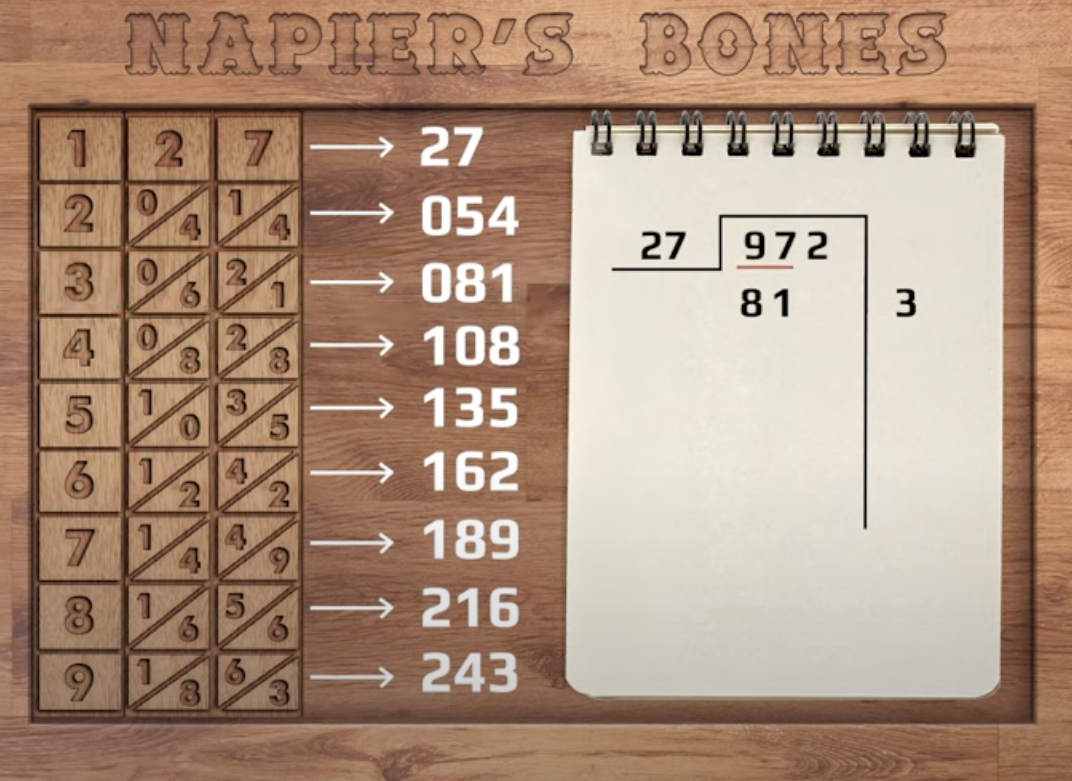
\includegraphics[width=0.8\linewidth]{napier.jpg}
		\caption{Napier's bones.}
	\end{figure}



\end{frame}

%------------------------------------------------

\begin{frame}
	\frametitle{Review: w1}

	\textbf{Input:} digit $x$ from 2-9, integer $n$ \\
\textbf{Output:} $x \times n$

\begin{enumerate}
    \item Arrange Napier's bones such that the first row corresponds to $n$.
    \item Write down the rightmost digit in the corresponding row.
    \item Add the two adjacent numbers and the carry digit in the same row to the left.
    \item Write down the ones place digit of the result from step 3.
    \item Carry the tens place digit from the result of step 3.
    \item Repeat steps 3-5 until you reach the leftmost column.
    \item Add the carry digit to the leftmost digit and write down the final result.
\end{enumerate}

\end{frame}

%------------------------------------------------

\begin{frame}
	\frametitle{Review: w1}

Linux is an open-source, Unix-like operating system that is widely used across various platforms such as servers, desktops, and embedded systems. Refer to:
\begin{itemize}
    \item \href{https://www.linuxfoundation.org/what-is-linux/}{[Link]}
\end{itemize}

\vspace{0.5cm}

The von Neumann architecture, is a computer architecture model that uses the same memory for storing both instructions and data. It consists of a central processing unit (CPU), memory, and input/output (I/O) units. The CPU retrieves instructions and data from memory, processdes them, and then sends results back to memory or I/O devices. Refer to:
\begin{itemize}
    \item \href{https://www.britannica.com/technology/von-Neumann-machine}{[Link]}
\end{itemize}


\end{frame}

%------------------------------------------------

\begin{frame}
	\frametitle{Review: w1}
Number system conversions are the process of converting numbers from one base to another. Refer to:
\begin{itemize}
    \item \href{https://www.geeksforgeeks.org/number-system-in-maths/}{[Link]}
\end{itemize}


	\begin{figure}
		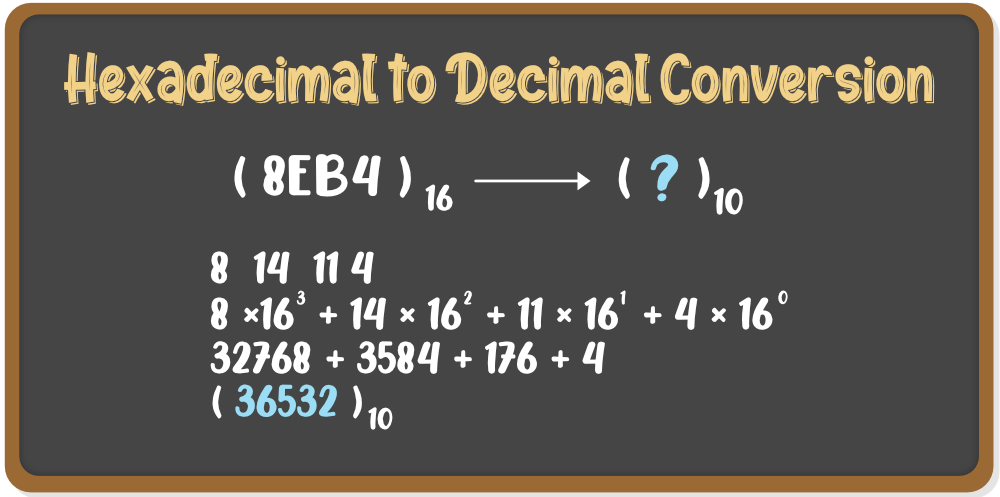
\includegraphics[width=0.8\linewidth]{hextodec.png}
	\end{figure}



\end{frame}

%------------------------------------------------

\begin{frame}
	\frametitle{Review: w1}

	\begin{figure}
		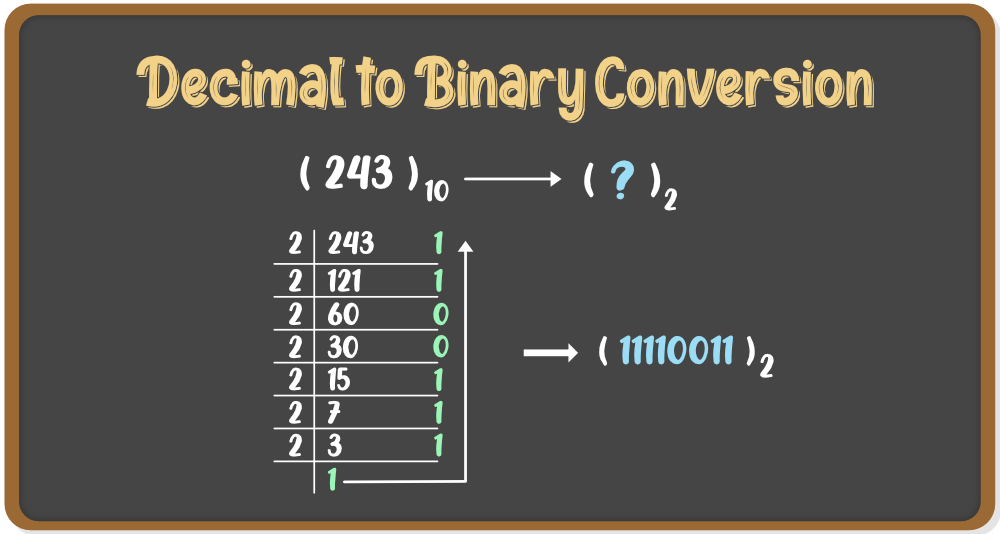
\includegraphics[width=0.6\linewidth]{dectobin.png}
	\end{figure}

	\begin{figure}
		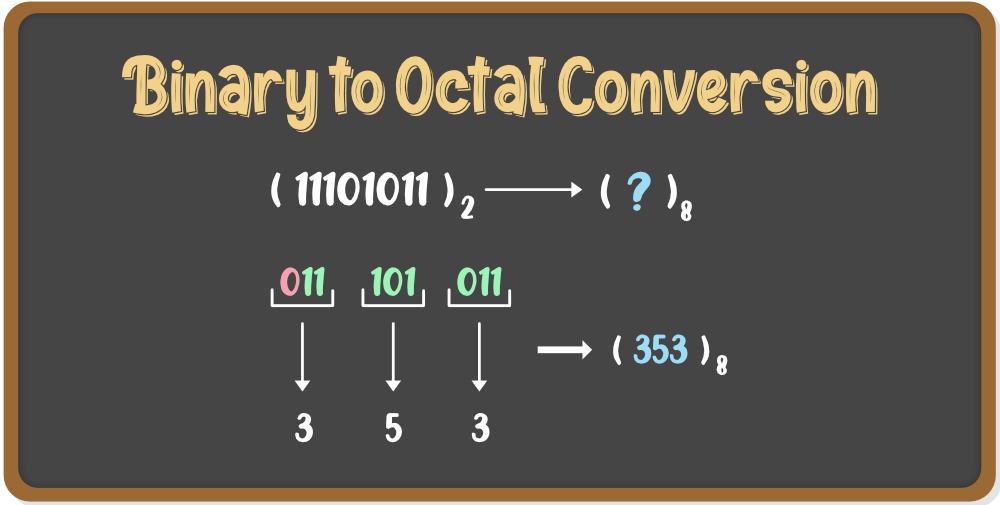
\includegraphics[width=0.6\linewidth]{bintooct.png}
	\end{figure}




\end{frame}

%------------------------------------------------

\begin{frame}
	\frametitle{Review: w1}
\textbf{Algorithm: Convert Decimal to Binary}

\textbf{Input:} digit $x$ \\
\textbf{Output:} $x$ in binary form

\begin{enumerate}
    \item Write down the remainder of $x$ divided by 2 (write the remainders from right to left).
    \item Update $x$: $x \leftarrow \lfloor x / 2 \rfloor$ (integer division).
    \item Repeat steps 1 and 2 until $x = 0$.
\end{enumerate}

\textbf{Example:} Convert 13 to binary.
\begin{itemize}
    \item $13 \div 2 = 6$, remainder = 1
    \item $6 \div 2 = 3$, remainder = 0
    \item $3 \div 2 = 1$, remainder = 1
    \item $1 \div 2 = 0$, remainder = 1
\end{itemize}

Reading the remainders from right to left, the binary representation of 13 is $1101_2$.




\end{frame}

%------------------------------------------------

\begin{frame}
	\frametitle{Review: w1}

	\textbf{Refer to:}
 
\hyperlink{slide:q7}{[Link]}

\begin{itemize}
    \item \textbf{Interpreted Language}: Python; Perl; PHP; Bash; Markdown; Ruby; Javascript
    \item \textbf{Compiled Language}: C\#; Ada95; O'Caml; Pascal; Fortran; Scala; Erlang
    \item \textbf{Interpreted/Compiled Language}: Haskell; Lisp
    \item \textbf{Compiled then Interpreted Language}: Java
    \item \textbf{Neither}: Assembly
\end{itemize}

\end{frame}

%------------------------------------------------

\subsection{w2}

\begin{frame}
	\frametitle{Review: w2}

\textbf{Graphical User Interface (GUI)}
It is a visual interface that allows users to interact with electronic devices using graphical elements such as icons, buttons, and windows. It is intuitive and easy to use, making it ideal for non-technical users.

\textbf{Command Line Interface (CLI)}
It is a text-based interface where users type commands to interact with the system. CLI offers greater control, precision, and speed for experienced users, making it a preferred tool for system administrators, developers, and engineers.

\end{frame}

%------------------------------------------------
\begin{frame}
	\frametitle{Review: w2}

	To start MATLAB in "No Desktop Mode" (headless mode), follow these steps:

	\begin{enumerate}
	    \item Open a terminal (CLI) on your system.
	    \item Start MATLAB in command-line mode using the following command (MacOS and Linux):
	    
	    \texttt{./matlab -nodisplay}
	    
	    \item Start MATLAB in command-line mode using the following command (Windows):
	    
	    \texttt{matlab -nosplash -nodesktop}
	\end{enumerate}

\end{frame}

%------------------------------------------------

\begin{frame}
	\frametitle{Review: w2}

	Rewrite the simple program from slide (2.6|2.60) using the 's' flag for the input function. Then convert the inputs from the 's' mode into into numbers.

\vspace{1.5cm}
\[
        num1 = input('Input \hspace{0.1cm} a \hspace{0.1cm} number: ','s');
\]

\[
        number1 = str2double(num1); \\
\]

\end{frame}

%------------------------------------------------

\begin{frame}
	\frametitle{Review: w2}

	\textbf{1. Generate a 10 × 10 matrix A composed of random elements.}
\[
A = \texttt{rand(10, 10)};
\]

\textbf{2. Extract the seventh element on the third row of A}

(i) Using its index:

 ( \text{index} = (row - 1) + (column - 1) \times \text{number of rows} + 1 )
 
\[
A(63);
\]
(ii) Using its coordinates:
\[
A(3, 7);
\]

\textbf{3. Delete the third column and the fourth row of A.}

\[
A1 = A([1:3 \hspace{0.15cm} 5:end],[1:2 \hspace{0.15cm} 4:end]);
\]


\end{frame}

%------------------------------------------------


\begin{frame}
	\frametitle{Review: w2}

	\textbf{4. Extract the sixth row and the second column from A.}
\[
row6 = A(6,:); 
\]
\[
col2 = A(:,2);
\]


\textbf{5. Extract the 4 × 4 matrix at the center of A.}
\[
A2 = A(4:7,4:7);
\]


\textbf{6. Construct the following matrix:}
\[
\begin{pmatrix}
A & A^T & B \\
A^T & A & C
\end{pmatrix}
\]
where B is the sum along of the rows of A and A′, and C is the subtraction of the sum of the rows of A with the sum of the rows of A′.
    \[
    B = sum(A,2)+sum((A'),2); disp(B); \]
    \[C = sum(A,2)-sum((A'),2); disp(C); \]


\end{frame}

%------------------------------------------------

\begin{frame}
	\frametitle{Review: w2}
\textbf{MATLAB Script: Truth Table for AND, OR, and XOR Operations}

\begin{verbatim}

A = [0 0 1 1]; \\
B = [0 1 0 1];

AND = A \& B; \% logical AND \\
OR = A | B; \% logical OR \\
XOR = xor(A, B); \% logical XOR \\

TT = [A; B; AND; OR; XOR]'; \\
disp('A B AND OR XOR'); \\
disp(TT); \\
\%      A      B      AND      OR      XOR \\
\%      0 \hspace{0.05cm}    0 \hspace{0.05cm}     0 \hspace{0.05cm}     0 \hspace{0.05cm}     0 \\
\%      0 \hspace{0.05cm}     1 \hspace{0.05cm}     0 \hspace{0.05cm}     1 \hspace{0.05cm}     1 \\
\%      1 \hspace{0.05cm}     0 \hspace{0.05cm}     0 \hspace{0.05cm}     1 \hspace{0.05cm}     1 \\
\%      1 \hspace{0.05cm}     1 \hspace{0.05cm}     1 \hspace{0.05cm}     1 \hspace{0.05cm}     0 \\
\end{verbatim}
\end{frame}

%------------------------------------------------
\begin{frame}
	\frametitle{Review: w2}

	\textbf{ASCII} stands for \textit{American Standard Code for Information Interchange}. It is a character encoding standard that assigns a numerical value to letters, digits, and punctuation, allowing text to be represented in computers.

 
	\begin{figure}
		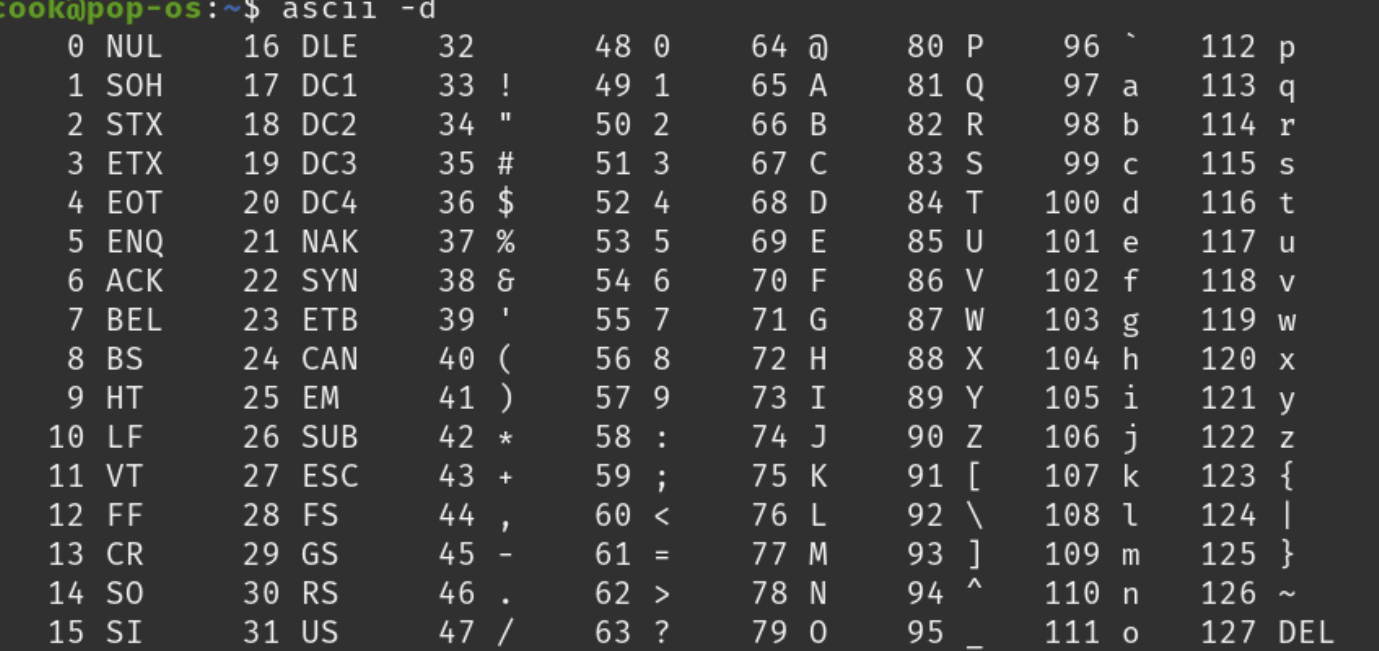
\includegraphics[width=0.7\linewidth]{ascii.png}
  		\caption{ASCII Table.\footnote{Source: https://www.johndcook.com/blog/2022/05/28/how-to-memorize-the-ascii-table/}}
	\end{figure}



\end{frame}

%------------------------------------------------


\begin{frame}
	\frametitle{Review: w2}

	\textbf{Algorithm: ASCII Code Lookup}

\textbf{Input:} A single character key \\
\textbf{Output:} ASCII code of the character

\begin{enumerate}
    \item Prompt the user to input a key.
    \item Check if the input length is exactly 1 character:
    \begin{itemize}
        \item If true:
        \begin{itemize}
            \item Convert the key to its ASCII code using the appropriate function. (eg. \texttt{double(key)})
            \item Display the ASCII code.
        \end{itemize}
        \item Else:
        \begin{itemize}
            \item Display an error message indicating the input is invalid.
        \end{itemize}
    \end{itemize}
\end{enumerate}

\textbf{Example 1: Valid Input}
\begin{itemize}
    \item Input: \texttt{A}
    \item Output: The ASCII code of \texttt{A} is 65
\end{itemize}

\textbf{Example 2: Invalid Input}
\begin{itemize}
    \item Input: \texttt{AB}
    \item Output: Invalid input. Please enter a single character.
\end{itemize}

\end{frame}

%------------------------------------------------


\begin{frame}
	\frametitle{Review: w2}

	\textbf{Algorithm: Count Vowels and Consonants}

\textbf{Input:} A word entered by the user \\
\textbf{Output:} Number of vowels and consonants in the word

\begin{enumerate}
    \item Initialize vowel\_count = 0
    \item Initialize consonant\_count = 0
    \item Define a set of vowels: \{a, e, i, o, u\}
    \item Prompt the user to input a word
    \item Convert the word to lowercase using the \texttt{lower()} function
    \item For each character in the word:
    \begin{itemize}
        \item If the character is in the vowels set:
        \begin{itemize}
            \item Increment vowel\_count
        \end{itemize}
        \item Else if the character is an alphabetic letter (check using \texttt{isletter()}):
        \begin{itemize}
            \item Increment consonant\_count
        \end{itemize}
    \end{itemize}
    \item Output the vowel\_count and consonant\_count
\end{enumerate}

\end{frame}

%------------------------------------------------



\begin{frame}
	\frametitle{Review: w2}

	\textbf{Generate a random 10×10 matrix, double all the elements less than 5, triple all the ones between 5 and 10, and set all the others to 0 if they are even or 1 if they are odd.}

\begin{enumerate}
    \item Generate a random 10x10 matrix with values between 0 and 20:
    \[
    M = randi([0, 20], 10, 10);
    M0 = M; % Keep a copy of the original matrix
    \]

    \item Double all the elements less than 5:
    \[
    M(M < 5) = M(M < 5) * 2;
    \]

    \item Triple all the elements between 5 and 10:
    \[
    M(M >= 5 \hspace{0.1cm} \& \hspace{0.1cm} M <= 10) = M(M >= 5 \hspace{0.1cm} \& \hspace{0.1cm} M <= 10) * 3;
    \]

    \item Set all the even elements greater than 10 to 0:
    \[
    M(mod(M0, 2) == 0 \hspace{0.1cm} \& \hspace{0.1cm} M0 > 10) = 0;
    \]

    \item Set all the odd elements greater than 10 to 1:
    \[
    M(mod(M0, 2) == 1 \hspace{0.1cm} \& \hspace{0.1cm} M0 > 10) = 1;
    \]
\end{enumerate}

\end{frame}

%------------------------------------------------

\begin{frame} % Use [allowframebreaks] to allow automatic splitting across slides if the content is too long
	\frametitle{References}
	
	\begin{itemize}
    \item Manuel. \textit{c1.pdf}. JI Canvas, 2024. \href{https://jicanvas.com/courses/917/files/folder/lectures?preview=333611}{[Link]}.

    \item Manuel. \textit{c2.pdf}. JI Canvas, 2024. \href{https://jicanvas.com/courses/917/files/folder/lectures?preview=333612}{[Link]}.

    \item Manuel. \textit{w1.pdf}. JI Canvas, 2024. \href{https://jicanvas.com/courses/917/files/folder/worksheets?preview=333629}{[Link]}.

    \item Manuel. \textit{w2.pdf}. JI Canvas, 2024. \href{https://jicanvas.com/courses/917/files/folder/worksheets?preview=333630}{[Link]}.

    \item Wang, Yuheng. \textit{RC-1.pdf}. JI Canvas, 2023. \href{https://jicanvas.com/courses/489/files/folder/rc?preview=223833}{[Link]}.

    \item Wang, Yuheng. \textit{rc}. FOCS JI Gitea, 2023. \href{https://focs.ji.sjtu.edu.cn/git/engr151-23fa/course-support/src/branch/master/rc}{[Link]}.
\end{itemize}
\end{frame}

%----------------------------------------------------------------------------------------
%	CLOSING SLIDE
%----------------------------------------------------------------------------------------

\begin{frame}[plain] % The optional argument 'plain' hides the headline and footline
	\begin{center}
		{\Huge The End}
		
		\bigskip\bigskip % Vertical whitespace
		
		{\LARGE Questions? Comments?}
	\end{center}
\end{frame}

%----------------------------------------------------------------------------------------

\end{document} 